\section{\emph{Batphone} : System Overview}\label{sec:overview}

Fig.~\ref{fig:batphone_vision} illustrates how the system will work.
\begin{figure}[h!t]
%\vspace{-0.1in}
\center{
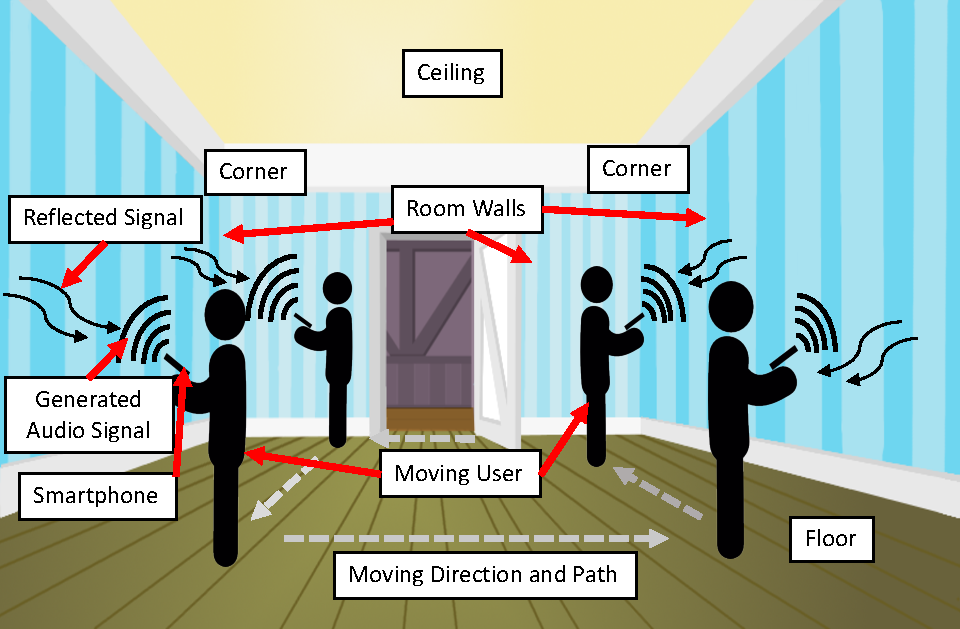
\includegraphics[width=\columnwidth]{figs/Batphone.pdf}
%\vspace{-0.1in}
\caption{{\small Batphone}}
%\vspace{-0.1in}
\label{fig:batphone_vision}
}
\end{figure}

Following are the building blocks coupled with their description :
\subsubsection{Dead Reckoning}
\begin{itemize}
\item Step size estimation
\item Step detection and count
\item Heading direction
\item Phone orientation
\end{itemize}

\subsubsection{FMCW based distance}
\begin{itemize}
\item FMCW parameter choices ( Chirp duration, Mic choice, Frequency response of speaker and mic based selection, Gap between chirps, Bandwidth selection, Sampling rate selection (Higher means lower quantization error or can also be done with zero padding). )
\item Synchronization with dead reckoning.
\item FMCW profile based corner detection and clutter filtering.
\end{itemize}

\subsubsection{Room shape profiling}
\begin{itemize}
\item Geometric constraints on the room wall and movement.
\item Corner detection help in profiling.
\end{itemize}